\documentclass[]{book}
\usepackage{lmodern}
\usepackage{amssymb,amsmath}
\usepackage{ifxetex,ifluatex}
\usepackage{fixltx2e} % provides \textsubscript
\ifnum 0\ifxetex 1\fi\ifluatex 1\fi=0 % if pdftex
  \usepackage[T1]{fontenc}
  \usepackage[utf8]{inputenc}
\else % if luatex or xelatex
  \ifxetex
    \usepackage{mathspec}
  \else
    \usepackage{fontspec}
  \fi
  \defaultfontfeatures{Ligatures=TeX,Scale=MatchLowercase}
\fi
% use upquote if available, for straight quotes in verbatim environments
\IfFileExists{upquote.sty}{\usepackage{upquote}}{}
% use microtype if available
\IfFileExists{microtype.sty}{%
\usepackage{microtype}
\UseMicrotypeSet[protrusion]{basicmath} % disable protrusion for tt fonts
}{}
\usepackage{hyperref}
\PassOptionsToPackage{usenames,dvipsnames}{color} % color is loaded by hyperref
\hypersetup{unicode=true,
            pdftitle={Skeleton Tutorial Template},
            pdfauthor={TJ McKinley},
            colorlinks=true,
            linkcolor=blue,
            citecolor=Blue,
            urlcolor=Blue,
            breaklinks=true}
\urlstyle{same}  % don't use monospace font for urls
\usepackage{color}
\usepackage{fancyvrb}
\newcommand{\VerbBar}{|}
\newcommand{\VERB}{\Verb[commandchars=\\\{\}]}
\DefineVerbatimEnvironment{Highlighting}{Verbatim}{commandchars=\\\{\}}
% Add ',fontsize=\small' for more characters per line
\usepackage{framed}
\definecolor{shadecolor}{RGB}{248,248,248}
\newenvironment{Shaded}{\begin{snugshade}}{\end{snugshade}}
\newcommand{\AlertTok}[1]{\textcolor[rgb]{0.94,0.16,0.16}{#1}}
\newcommand{\AnnotationTok}[1]{\textcolor[rgb]{0.56,0.35,0.01}{\textbf{\textit{#1}}}}
\newcommand{\AttributeTok}[1]{\textcolor[rgb]{0.77,0.63,0.00}{#1}}
\newcommand{\BaseNTok}[1]{\textcolor[rgb]{0.00,0.00,0.81}{#1}}
\newcommand{\BuiltInTok}[1]{#1}
\newcommand{\CharTok}[1]{\textcolor[rgb]{0.31,0.60,0.02}{#1}}
\newcommand{\CommentTok}[1]{\textcolor[rgb]{0.56,0.35,0.01}{\textit{#1}}}
\newcommand{\CommentVarTok}[1]{\textcolor[rgb]{0.56,0.35,0.01}{\textbf{\textit{#1}}}}
\newcommand{\ConstantTok}[1]{\textcolor[rgb]{0.00,0.00,0.00}{#1}}
\newcommand{\ControlFlowTok}[1]{\textcolor[rgb]{0.13,0.29,0.53}{\textbf{#1}}}
\newcommand{\DataTypeTok}[1]{\textcolor[rgb]{0.13,0.29,0.53}{#1}}
\newcommand{\DecValTok}[1]{\textcolor[rgb]{0.00,0.00,0.81}{#1}}
\newcommand{\DocumentationTok}[1]{\textcolor[rgb]{0.56,0.35,0.01}{\textbf{\textit{#1}}}}
\newcommand{\ErrorTok}[1]{\textcolor[rgb]{0.64,0.00,0.00}{\textbf{#1}}}
\newcommand{\ExtensionTok}[1]{#1}
\newcommand{\FloatTok}[1]{\textcolor[rgb]{0.00,0.00,0.81}{#1}}
\newcommand{\FunctionTok}[1]{\textcolor[rgb]{0.00,0.00,0.00}{#1}}
\newcommand{\ImportTok}[1]{#1}
\newcommand{\InformationTok}[1]{\textcolor[rgb]{0.56,0.35,0.01}{\textbf{\textit{#1}}}}
\newcommand{\KeywordTok}[1]{\textcolor[rgb]{0.13,0.29,0.53}{\textbf{#1}}}
\newcommand{\NormalTok}[1]{#1}
\newcommand{\OperatorTok}[1]{\textcolor[rgb]{0.81,0.36,0.00}{\textbf{#1}}}
\newcommand{\OtherTok}[1]{\textcolor[rgb]{0.56,0.35,0.01}{#1}}
\newcommand{\PreprocessorTok}[1]{\textcolor[rgb]{0.56,0.35,0.01}{\textit{#1}}}
\newcommand{\RegionMarkerTok}[1]{#1}
\newcommand{\SpecialCharTok}[1]{\textcolor[rgb]{0.00,0.00,0.00}{#1}}
\newcommand{\SpecialStringTok}[1]{\textcolor[rgb]{0.31,0.60,0.02}{#1}}
\newcommand{\StringTok}[1]{\textcolor[rgb]{0.31,0.60,0.02}{#1}}
\newcommand{\VariableTok}[1]{\textcolor[rgb]{0.00,0.00,0.00}{#1}}
\newcommand{\VerbatimStringTok}[1]{\textcolor[rgb]{0.31,0.60,0.02}{#1}}
\newcommand{\WarningTok}[1]{\textcolor[rgb]{0.56,0.35,0.01}{\textbf{\textit{#1}}}}
\usepackage{longtable,booktabs}
\usepackage{graphicx,grffile}
\makeatletter
\def\maxwidth{\ifdim\Gin@nat@width>\linewidth\linewidth\else\Gin@nat@width\fi}
\def\maxheight{\ifdim\Gin@nat@height>\textheight\textheight\else\Gin@nat@height\fi}
\makeatother
% Scale images if necessary, so that they will not overflow the page
% margins by default, and it is still possible to overwrite the defaults
% using explicit options in \includegraphics[width, height, ...]{}
\setkeys{Gin}{width=\maxwidth,height=\maxheight,keepaspectratio}
\IfFileExists{parskip.sty}{%
\usepackage{parskip}
}{% else
\setlength{\parindent}{0pt}
\setlength{\parskip}{6pt plus 2pt minus 1pt}
}
\setlength{\emergencystretch}{3em}  % prevent overfull lines
\providecommand{\tightlist}{%
  \setlength{\itemsep}{0pt}\setlength{\parskip}{0pt}}
\setcounter{secnumdepth}{5}
% Redefines (sub)paragraphs to behave more like sections
\ifx\paragraph\undefined\else
\let\oldparagraph\paragraph
\renewcommand{\paragraph}[1]{\oldparagraph{#1}\mbox{}}
\fi
\ifx\subparagraph\undefined\else
\let\oldsubparagraph\subparagraph
\renewcommand{\subparagraph}[1]{\oldsubparagraph{#1}\mbox{}}
\fi

%%% Use protect on footnotes to avoid problems with footnotes in titles
\let\rmarkdownfootnote\footnote%
\def\footnote{\protect\rmarkdownfootnote}

%%% Change title format to be more compact
\usepackage{titling}

% Create subtitle command for use in maketitle
\providecommand{\subtitle}[1]{
  \posttitle{
    \begin{center}\large#1\end{center}
    }
}

\setlength{\droptitle}{-2em}

  \title{Skeleton Tutorial Template}
    \pretitle{\vspace{\droptitle}\centering\huge}
  \posttitle{\par}
    \author{TJ McKinley}
    \preauthor{\centering\large\emph}
  \postauthor{\par}
    \date{}
    \predate{}\postdate{}
  
% latex macro to create task boxes
\usepackage{tcolorbox, comment}
\tcbuselibrary{breakable}

\definecolor{taskCol}{HTML}{404040}
\definecolor{taskCol1}{HTML}{808080}

\tcbset{colback=white,colframe=taskCol,arc=0mm}

%trick to fool markdown into compiling
\newcommand{\bblockT}[2][Task]{\begin{tcolorbox}[title = #1 #2, parbox = false]}
\newcommand{\eblockT}{\end{tcolorbox}}
\newcommand{\bblockS}[2][Solution]{\begin{tcolorbox}[title = #1 #2, colframe=taskCol1, breakable, parbox = false]}
\newcommand{\eblockS}{\end{tcolorbox}}

%add tabbed solutions environment
\newcommand{\bmp}{\begin{minipage}[c]{0.5\textwidth}}
\newcommand{\emp}{\end{minipage}}
\newcommand{\bblockST}[1]{\begin{tcolorbox}[title = #1, colframe=taskCol1, breakable, parbox = false]}
\newcommand{\eblockST}{\end{tcolorbox}}

%set solution button link
\usepackage{tikz}

\newcommand{\buttonT}[1]{
    \begin{tikzpicture}
    \node[
        inner sep=5pt,
        draw=taskCol,
        fill=taskCol,
        rounded corners=2pt,
        text=white
    ] (c1) {#1};
    \end{tikzpicture}
}

\newcommand{\buttonS}[1]{
    \begin{tikzpicture}
    \node[
        inner sep=5pt,
        draw=taskCol1,
        fill=taskCol1,
        rounded corners=2pt,
        text=white
    ] (c1) {#1};
    \end{tikzpicture}
}

\newcommand{\colpageref}[1]{\hypersetup{linkcolor=white}\pageref{#1}}

\begin{document}
\maketitle

{
\hypersetup{linkcolor=black}
\setcounter{tocdepth}{1}
\tableofcontents
}
\hypertarget{opening-page}{%
\chapter{Opening page}\label{opening-page}}

Basically a standard Bookdown template with a few tweaks. New chapters need to be in separate `.Rmd' files, where each file starts with a chapter heading as seen \href{https://bookdown.org/yihui/bookdown/usage.html}{here}. In order to use the task and solution blocks in \LaTeX, you must input the order of the files into the \texttt{\_bookdown.yml} file, and the first file must be called \texttt{index.Rmd} e.g.

\begin{verbatim}
rmd_files:
    html: ['index.Rmd', 'ch1.Rmd']
    latex: ['index.Rmd', 'ch1.Rmd', 'ch_appendix.Rmd']
output_dir: "docs"
\end{verbatim}

The \texttt{latex:} path above \textbf{\emph{must}} have \texttt{\textquotesingle{}ch\_appendix.Rmd\textquotesingle{}} as its last entry. This ensures that the appendix is properly formatted for the solutions to the problems.

There are a couple of useful special blocks. A \texttt{task} block, and a \texttt{solution} block. These can be used as e.g.

\begin{verbatim}
```{task}
Here is a task written in **markdown**.
```
\end{verbatim}

which renders as:

\hypertarget{tsk1}{}\bblockT[Task]{\phantomsection\label{sol1}1}

Here is a task written in \textbf{markdown}.
\eblockT

You can include chunks within the \texttt{task} chunk, but you need to use double backticks \emph{within} the chunk, and leave carriage returns around the internal chunk e.g.

\begin{verbatim}

```{task}

``{r}
x <- 2 + 2
x
``

```
\end{verbatim}

which renders as:

\hypertarget{tsk2}{}\bblockT[Task]{\phantomsection\label{sol2}2}

\begin{Shaded}
\begin{Highlighting}[]
\NormalTok{x <-}\StringTok{ }\DecValTok{2} \OperatorTok{+}\StringTok{ }\DecValTok{2}
\NormalTok{x}
\end{Highlighting}
\end{Shaded}

\begin{verbatim}
## [1] 4
\end{verbatim}

\eblockT

Be careful to have suitable carriage returns around e.g.~\texttt{enumerate} or \texttt{itemize} environments inside the chunk also. For example:

\begin{verbatim}

```{task}
Here is a list:
1. item 1
2. item 2
```
\end{verbatim}

will not render nicely. But

\begin{verbatim}

```{task}
Here is a list:

1. item 1
2. item 2

```
\end{verbatim}

will:

\hypertarget{tsk3}{}\bblockT[Task]{\phantomsection\label{sol3}3}

Here is a list:

\begin{enumerate}
\def\labelenumi{\arabic{enumi}.}
\tightlist
\item
  item 1
\item
  item 2
\end{enumerate}

\eblockT

The \texttt{solution} chunk works in the same way, and the numbers will follow the previous \texttt{task} chunk (so you can set tasks without solutions) e.g.

\begin{verbatim}

```{task}
Add 2 and 2 together
```

```{solution}

``{r}
2 + 2
``

```
\end{verbatim}

gives:

\hypertarget{tsk4}{}\bblockT[Task]{\phantomsection\label{sol4}4}

Add 2 and 2 together
\eblockT

\hyperlink{sol4}{\buttonS{Show Solution on P\colpageref{tsk4}}}

To compile, run the \texttt{\_build.sh} script which will compile into multiple formats.

\hypertarget{additional-extensions}{%
\section{Additional extensions}\label{additional-extensions}}

\hypertarget{different-task-and-solution-titles}{%
\subsection{Different task and solution titles}\label{different-task-and-solution-titles}}

Task and solution boxes can also be given different names using the \texttt{title} option e.g.

\begin{verbatim}

```{task, title = "Question"}
What is the meaning of life, the universe and everything?
```

```{solution, title = "Answer"}
Why 42 of course!
```
\end{verbatim}

gives:

\hypertarget{tsk5}{}\bblockT[Question]{\phantomsection\label{sol5}5}

What is the meaning of life, the universe and everything?
\eblockT

\hyperlink{sol5}{\buttonS{Show Answer on P\colpageref{tsk5}}}

\hypertarget{tabbed-boxed-environments}{%
\subsection{Tabbed boxed environments}\label{tabbed-boxed-environments}}

Originally developed to put base R and \texttt{tidyverse} solutions side-by-side, using a \texttt{multCode\ =\ T} option to the solution box. Here the two tabs are separated by four consecutive hashes: \texttt{\#\#\#\#}, and the \texttt{titles} option gives the tab titles (these can be set globally if preferred) e.g.

\begin{verbatim}

```{task}
Filter the `iris` data by `Species == "setosa"` and find the mean `Petal.Length`.
```

```{solution, multCode = T, titles = c("Base R", "tidyverse")}

``{r}
## base R solution
mean(iris$Petal.Length[
    iris$Species == "setosa"])
``

####

``{r}
## tidyverse solution
iris %>% 
    filter(Species == "setosa") %>%
    select(Petal.Length) %>%
    summarise(mean = mean(Petal.Length))
``
    
```
\end{verbatim}

will typeset to:

\hypertarget{tsk6}{}\bblockT[Task]{\phantomsection\label{sol6}6}

Filter the \texttt{iris} data by \texttt{Species\ ==\ "setosa"} and find the mean \texttt{Petal.Length}.
\eblockT

\hyperlink{sol6}{\buttonS{Show Solution on P\colpageref{tsk6}}}

Note that there is also a \texttt{multCode} chunk that does not link to task and solution boxes e.g.

\begin{verbatim}

```{multCode}

Two options: 

* Option 1

####

Two options:
    
* Option 2

```
\end{verbatim}

will typeset to:

\bmp
\bblockST{Option 1}

Two options:

\begin{itemize}
\tightlist
\item
  Option 1
\end{itemize}

\eblockST
\emp
\hspace{0.01\textwidth}
\bmp\bblockST{Option 2}

Two options:

\begin{itemize}
\tightlist
\item
  Option 2
\end{itemize}

\eblockST
\emp

The \texttt{titles} option can be set as before.

\hypertarget{hello-world}{%
\chapter{Hello, world!}\label{hello-world}}

\hypertarget{importing-vector-data}{%
\section{Importing vector data}\label{importing-vector-data}}

\hypertarget{spatial-data-formats}{%
\subsection{Spatial data formats}\label{spatial-data-formats}}

The \href{https://gdal.org/}{Geospatial Data Abstraction Library} is a translator library for raster and vector geospatial data formats. We will start by loading the R package of this library and check all the vector data formats that can be imported into R

\begin{Shaded}
\begin{Highlighting}[]
\KeywordTok{library}\NormalTok{(rgdal)}
\NormalTok{vector_formats <-}\StringTok{ }\KeywordTok{ogrDrivers}\NormalTok{()}
\KeywordTok{head}\NormalTok{(vector_formats)}
\end{Highlighting}
\end{Shaded}

\begin{verbatim}
##         name                     long_name write  copy isVector
## 1 AeronavFAA                   Aeronav FAA FALSE FALSE     TRUE
## 2 AmigoCloud                    AmigoCloud  TRUE FALSE     TRUE
## 3     ARCGEN             Arc/Info Generate FALSE FALSE     TRUE
## 4     AVCBin      Arc/Info Binary Coverage FALSE FALSE     TRUE
## 5     AVCE00 Arc/Info E00 (ASCII) Coverage FALSE FALSE     TRUE
## 6        BNA                     Atlas BNA  TRUE FALSE     TRUE
\end{verbatim}

You can explore \texttt{vector\_formats}. How many different formats are available? Are you familiar with any of them?

\hypertarget{import-shapefiles}{%
\subsection{Import shapefiles}\label{import-shapefiles}}

\href{https://en.wikipedia.org/wiki/Shapefile}{shapefile} is a popular format used in GIS.
We will import a polygon layer of the world countries extracted from \href{https://www.naturalearthdata.com/}{Natural Earth}.

\begin{Shaded}
\begin{Highlighting}[]
\CommentTok{# Import countries}
\NormalTok{countries <-}\StringTok{ }\KeywordTok{readOGR}\NormalTok{(}\DataTypeTok{dsn =} \StringTok{"data/ne/ne_110m_admin_0_countries"}\NormalTok{, }\DataTypeTok{layer =} \StringTok{"ne_110m_admin_0_countries"}\NormalTok{)}
\end{Highlighting}
\end{Shaded}

\begin{verbatim}
## OGR data source with driver: ESRI Shapefile 
## Source: "C:\Git\skeleton_Rmd-master\data\ne\ne_110m_admin_0_countries", layer: "ne_110m_admin_0_countries"
## with 177 features
## It has 94 fields
## Integer64 fields read as strings:  POP_EST NE_ID
\end{verbatim}

We can check the class and spatial attributes of this layer

\begin{Shaded}
\begin{Highlighting}[]
\CommentTok{# View spatial attributes}
\KeywordTok{class}\NormalTok{(countries)  }\CommentTok{# sp class}
\end{Highlighting}
\end{Shaded}

\begin{verbatim}
## [1] "SpatialPolygonsDataFrame"
## attr(,"package")
## [1] "sp"
\end{verbatim}

And now, let's make our first plot using base R graphics

\begin{Shaded}
\begin{Highlighting}[]
\CommentTok{# Quick plot}
\KeywordTok{plot}\NormalTok{(countries, }\DataTypeTok{main =} \StringTok{"World countries"}\NormalTok{)}
\end{Highlighting}
\end{Shaded}

\begin{center}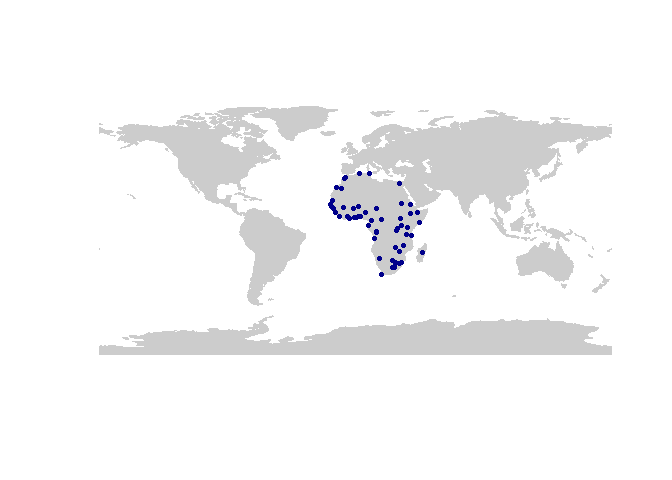
\includegraphics{_main_files/figure-latex/unnamed-chunk-16-1} \end{center}

\hypertarget{coordinate-reference-systems-crs}{%
\section{Coordinate Reference Systems (CRS)}\label{coordinate-reference-systems-crs}}

You can check the CRS from your spatial object

\begin{Shaded}
\begin{Highlighting}[]
\CommentTok{# View spatial attributes}
\KeywordTok{proj4string}\NormalTok{(countries)  }\CommentTok{# displays the coordinate reference system (CRS)}
\end{Highlighting}
\end{Shaded}

\begin{verbatim}
## [1] "+proj=longlat +datum=WGS84 +no_defs +ellps=WGS84 +towgs84=0,0,0"
\end{verbatim}

And then transform to another CRS. In this case, we transform to the \href{https://en.wikipedia.org/wiki/Mollweide_projection}{Mollweide projection}. This is an accurate single global projection that preserves geographic area. You can see an example of application in \href{https://doi.org/10.1111/gcb.14902}{March et al.~2019}

\begin{Shaded}
\begin{Highlighting}[]
\CommentTok{# Change to Mollweide projection}
\NormalTok{countries_moll <-}\StringTok{ }\KeywordTok{spTransform}\NormalTok{(countries, }\KeywordTok{CRS}\NormalTok{(}\StringTok{"+proj=moll +ellps=WGS84"}\NormalTok{))}

\CommentTok{# Quick plot}
\KeywordTok{plot}\NormalTok{(countries_moll, }\DataTypeTok{col =} \StringTok{"grey80"}\NormalTok{, }\DataTypeTok{main =} \StringTok{"World countries"}\NormalTok{)}
\end{Highlighting}
\end{Shaded}

\begin{center}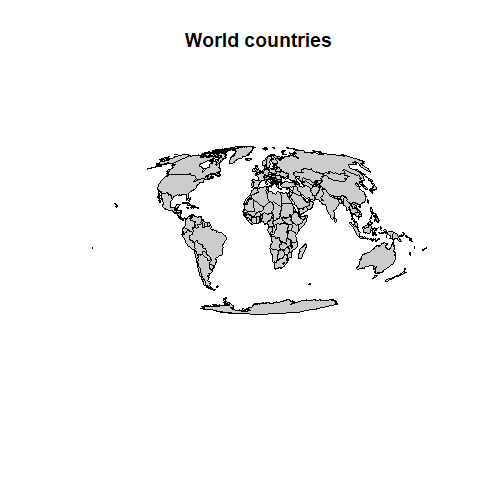
\includegraphics{_main_files/figure-latex/unnamed-chunk-18-1} \end{center}

\hypertarget{geographic-subset}{%
\section{Geographic subset}\label{geographic-subset}}

\hypertarget{geographic-subset-by-setting-a-bounding-box}{%
\subsection{Geographic subset by setting a bounding box}\label{geographic-subset-by-setting-a-bounding-box}}

First, create a bounding area for subsetting the data

\begin{Shaded}
\begin{Highlighting}[]
\CommentTok{# Import raster package}
\KeywordTok{library}\NormalTok{(raster)}

\CommentTok{# Set min and maximum coordinates (lon/lat)}
\NormalTok{xmin <-}\StringTok{ }\DecValTok{-15}
\NormalTok{xmax <-}\StringTok{ }\DecValTok{46}
\NormalTok{ymin <-}\StringTok{ }\DecValTok{28}
\NormalTok{ymax <-}\StringTok{ }\DecValTok{60}

\CommentTok{# Create an extent object}
\NormalTok{e <-}\StringTok{ }\KeywordTok{extent}\NormalTok{(xmin, xmax, ymin, ymax)}
\KeywordTok{class}\NormalTok{(e)}
\end{Highlighting}
\end{Shaded}

\begin{verbatim}
## [1] "Extent"
## attr(,"package")
## [1] "raster"
\end{verbatim}

Then, you can use the \texttt{extent} object to subset the worl map using \texttt{crop()} function

\begin{Shaded}
\begin{Highlighting}[]
\CommentTok{# Geographic subset of countries by the extent defined}
\NormalTok{countries_subset <-}\StringTok{ }\KeywordTok{crop}\NormalTok{(countries, e)}
\KeywordTok{plot}\NormalTok{(countries_subset)}
\end{Highlighting}
\end{Shaded}

\begin{center}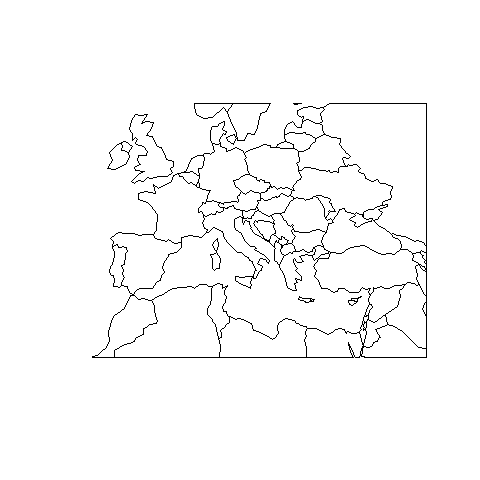
\includegraphics{_main_files/figure-latex/unnamed-chunk-20-1} \end{center}

\hypertarget{exercise}{%
\subsubsection{Exercise:}\label{exercise}}

\begin{itemize}
\tightlist
\item
  Make a plot of South America
\item
  Tip: you can Use QGIS or Google Earth to search for coordinates
\end{itemize}

\hypertarget{geographic-subset-by-data-attributes}{%
\subsection{Geographic subset by data attributes}\label{geographic-subset-by-data-attributes}}

The spatial layer of polygons has a linked attribute table, with specific information for each country. You can explore convert the \texttt{@data} object from \texttt{countries} into a \texttt{data.frame} and then explore the attribute data.

\begin{Shaded}
\begin{Highlighting}[]
\CommentTok{# Convert attribute data into a data.frame}
\NormalTok{df <-}\StringTok{ }\KeywordTok{data.frame}\NormalTok{(countries}\OperatorTok{@}\NormalTok{data)}
\CommentTok{# head(df)}
\end{Highlighting}
\end{Shaded}

List of continents

\begin{Shaded}
\begin{Highlighting}[]
\KeywordTok{unique}\NormalTok{(countries}\OperatorTok{$}\NormalTok{CONTINENT)}
\end{Highlighting}
\end{Shaded}

\begin{verbatim}
## [1] Oceania                 Africa                  North America          
## [4] Asia                    South America           Europe                 
## [7] Seven seas (open ocean) Antarctica             
## 8 Levels: Africa Antarctica Asia Europe North America ... South America
\end{verbatim}

Subset countries from South America

\begin{Shaded}
\begin{Highlighting}[]
\CommentTok{# Subset South America}
\NormalTok{south_america <-}\StringTok{ }\NormalTok{countries[countries}\OperatorTok{$}\NormalTok{CONTINENT }\OperatorTok{==}\StringTok{ "South America"}\NormalTok{,]}
\KeywordTok{plot}\NormalTok{(south_america, }\DataTypeTok{col =} \StringTok{"lightgreen"}\NormalTok{, }\DataTypeTok{border =} \StringTok{"darkgreen"}\NormalTok{, }\DataTypeTok{lwd=}\DecValTok{3}\NormalTok{, }\DataTypeTok{main =} \StringTok{"South America"}\NormalTok{)}
\end{Highlighting}
\end{Shaded}

\begin{center}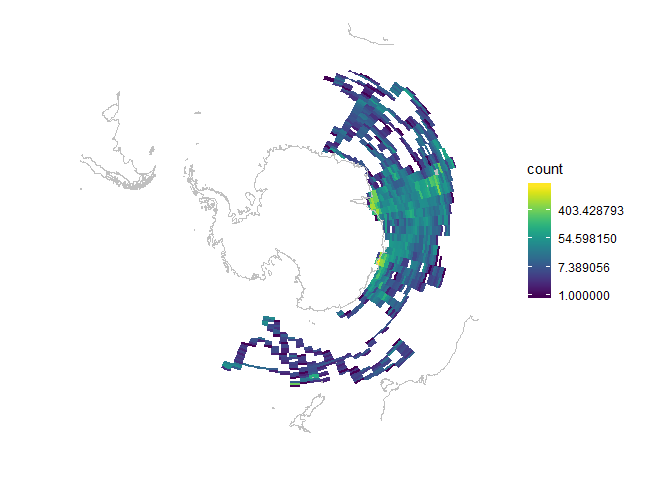
\includegraphics{_main_files/figure-latex/unnamed-chunk-23-1} \end{center}

\begin{Shaded}
\begin{Highlighting}[]
\KeywordTok{extent}\NormalTok{(south_america)  }\CommentTok{# You can also get your extent}
\end{Highlighting}
\end{Shaded}

\begin{verbatim}
## class      : Extent 
## xmin       : -81.41094 
## xmax       : -34.72999 
## ymin       : -55.61183 
## ymax       : 12.4373
\end{verbatim}

\hypertarget{import-vector-layer-point-data}{%
\section{Import vector layer: point data}\label{import-vector-layer-point-data}}

We will import layer ``Populated places of the world'' from Natural Earth

\begin{Shaded}
\begin{Highlighting}[]
\CommentTok{# Import populated places}
\NormalTok{places <-}\StringTok{ }\KeywordTok{readOGR}\NormalTok{(}\DataTypeTok{dsn =} \StringTok{"data/ne/ne_110m_populated_places_simple"}\NormalTok{, }\DataTypeTok{layer =} \StringTok{"ne_110m_populated_places_simple"}\NormalTok{)}
\end{Highlighting}
\end{Shaded}

\begin{verbatim}
## OGR data source with driver: ESRI Shapefile 
## Source: "C:\Git\skeleton_Rmd-master\data\ne\ne_110m_populated_places_simple", layer: "ne_110m_populated_places_simple"
## with 243 features
## It has 38 fields
## Integer64 fields read as strings:  ne_id
\end{verbatim}

\begin{Shaded}
\begin{Highlighting}[]
\CommentTok{# View spatial attributes}
\KeywordTok{class}\NormalTok{(places)}
\end{Highlighting}
\end{Shaded}

\begin{verbatim}
## [1] "SpatialPointsDataFrame"
## attr(,"package")
## [1] "sp"
\end{verbatim}

\begin{Shaded}
\begin{Highlighting}[]
\KeywordTok{extent}\NormalTok{(places)}
\end{Highlighting}
\end{Shaded}

\begin{verbatim}
## class      : Extent 
## xmin       : -175.2206 
## xmax       : 179.2166 
## ymin       : -41.29999 
## ymax       : 64.15002
\end{verbatim}

\begin{Shaded}
\begin{Highlighting}[]
\KeywordTok{crs}\NormalTok{(places)}
\end{Highlighting}
\end{Shaded}

\begin{verbatim}
## CRS arguments:
##  +proj=longlat +datum=WGS84 +no_defs +ellps=WGS84 +towgs84=0,0,0
\end{verbatim}

\begin{Shaded}
\begin{Highlighting}[]
\CommentTok{# Quick plot}
\KeywordTok{plot}\NormalTok{(places, }\DataTypeTok{main =} \StringTok{"Populated places"}\NormalTok{)  }
\end{Highlighting}
\end{Shaded}

\begin{center}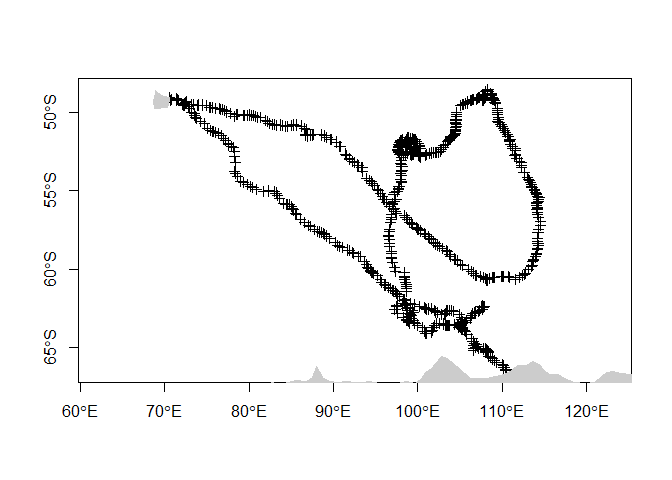
\includegraphics{_main_files/figure-latex/unnamed-chunk-24-1} \end{center}

The plot is not very informative. Let's combine with the world map

\begin{Shaded}
\begin{Highlighting}[]
\CommentTok{# Plot together with country maps}
\KeywordTok{plot}\NormalTok{(countries, }\DataTypeTok{col =} \StringTok{"grey80"}\NormalTok{, }\DataTypeTok{border =} \StringTok{"grey80"}\NormalTok{)}
\KeywordTok{plot}\NormalTok{(places, }\DataTypeTok{pch =} \DecValTok{20}\NormalTok{, }\DataTypeTok{col =} \StringTok{"darkblue"}\NormalTok{, }\DataTypeTok{add =} \OtherTok{TRUE}\NormalTok{)}
\end{Highlighting}
\end{Shaded}

\begin{center}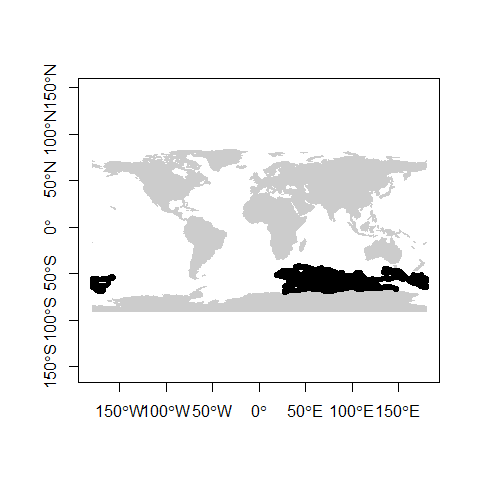
\includegraphics{_main_files/figure-latex/unnamed-chunk-25-1} \end{center}

\hypertarget{spatial-overlap}{%
\section{Spatial overlap}\label{spatial-overlap}}

The overlap between spatial layer in order to extract information from one to another is one of the most common tasks in GIS.

Here, we want to plot the populated places from Europe. However, there is no information about the continent in the places layer. We will use a spatial overlay to extract information from the countries layer using the function \texttt{over()}

\begin{Shaded}
\begin{Highlighting}[]
\CommentTok{# Spatial overlay}
\NormalTok{ov <-}\StringTok{ }\KeywordTok{over}\NormalTok{(places, countries)}
\KeywordTok{class}\NormalTok{(ov)}
\end{Highlighting}
\end{Shaded}

\begin{verbatim}
## [1] "data.frame"
\end{verbatim}

We then can append the continent information into the point layer

\begin{Shaded}
\begin{Highlighting}[]
\NormalTok{places}\OperatorTok{$}\NormalTok{CONTINENT <-}\StringTok{ }\NormalTok{ov}\OperatorTok{$}\NormalTok{CONTINENT}
\CommentTok{# head(places)}
\end{Highlighting}
\end{Shaded}

Note that there are places with \texttt{NA} in the continent attribute. This is due to a spatial missmatch between layers in terms of resolution, more specifically because of the coarse resolution of the countries layer. There would be several alternatives: 1) use a high-res countries map, 2) calculate the nearest polygon.

\begin{Shaded}
\begin{Highlighting}[]
\CommentTok{# Subset places and countries from Africa}
\NormalTok{places_africa <-}\StringTok{ }\NormalTok{places[}\KeywordTok{which}\NormalTok{(places}\OperatorTok{$}\NormalTok{CONTINENT }\OperatorTok{==}\StringTok{ "Africa"}\NormalTok{),]}

\CommentTok{# Plot together with country maps}
\KeywordTok{plot}\NormalTok{(countries, }\DataTypeTok{col =} \StringTok{"grey80"}\NormalTok{, }\DataTypeTok{border =} \StringTok{"grey80"}\NormalTok{)}
\KeywordTok{plot}\NormalTok{(places_africa, }\DataTypeTok{pch =} \DecValTok{20}\NormalTok{, }\DataTypeTok{col =} \StringTok{"darkblue"}\NormalTok{, }\DataTypeTok{add =} \OtherTok{TRUE}\NormalTok{)}
\end{Highlighting}
\end{Shaded}

\begin{center}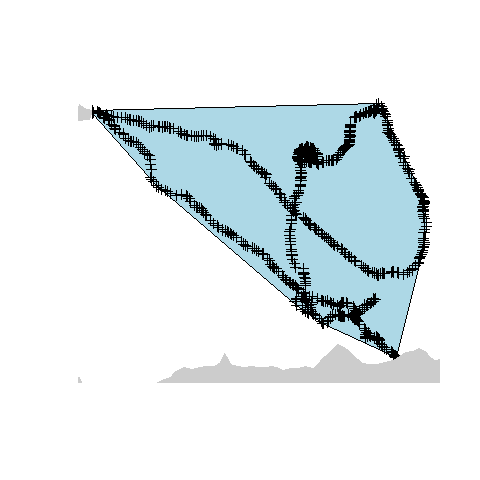
\includegraphics{_main_files/figure-latex/unnamed-chunk-28-1} \end{center}

\hypertarget{interactive-maps}{%
\section{Interactive maps}\label{interactive-maps}}

Spatial datasets oftern require to conduct an interative visualization of the data. In R, we can use the \texttt{leaflet} library to generate a dynamic viewer.

\begin{Shaded}
\begin{Highlighting}[]
\CommentTok{# import leaflet package}
\KeywordTok{library}\NormalTok{(leaflet)}

\CommentTok{# create leaftet map}
\NormalTok{map <-}\StringTok{ }\KeywordTok{leaflet}\NormalTok{(}\DataTypeTok{data =}\NormalTok{ places) }\OperatorTok
\StringTok{  }\KeywordTok{addProviderTiles}\NormalTok{(}\StringTok{"Esri.OceanBasemap"}\NormalTok{) }\OperatorTok\StringTok{  }\CommentTok{# Base map}
\StringTok{  }\KeywordTok{addMarkers}\NormalTok{(}\DataTypeTok{popup =} \OperatorTok{~}\NormalTok{name)}

\CommentTok{# plot leaflet map}
\CommentTok{# map}
\end{Highlighting}
\end{Shaded}

You can customize your map using different basemaps, add more spatial layers and much more. You can check the \href{https://rstudio.github.io/leaflet/}{official package website} for many examples

\newgeometry{margin=0.5in}

\hypertarget{appendix-appendix}{%
\appendix}


\hypertarget{answers}{%
\chapter{Answers}\label{answers}}

\hypertarget{sol4}{}
\bblockS[Solution]{\phantomsection\label{tsk4}4}

\begin{Shaded}
\begin{Highlighting}[]
\DecValTok{2} \OperatorTok{+}\StringTok{ }\DecValTok{2}
\end{Highlighting}
\end{Shaded}

\begin{verbatim}
## [1] 4
\end{verbatim}

\vspace{\baselineskip}

\hyperlink{tsk4}{\buttonT{Return to task on P\colpageref{sol4}}}
\eblockS
\hypertarget{sol5}{}
\bblockS[Answer]{\phantomsection\label{tsk5}5}

Why 42 of course!

\vspace{\baselineskip}

\hyperlink{tsk5}{\buttonT{Return to task on P\colpageref{sol5}}}
\eblockS
\hypertarget{sol6}{}
\bblockS[Solution]{\phantomsection\label{tsk6}6}
\bmp
\bblockST{Base R}

\begin{Shaded}
\begin{Highlighting}[]
\CommentTok{## base R solution}
\KeywordTok{mean}\NormalTok{(iris}\OperatorTok{$}\NormalTok{Petal.Length[}
\NormalTok{    iris}\OperatorTok{$}\NormalTok{Species }\OperatorTok{==}\StringTok{ "setosa"}\NormalTok{])}
\end{Highlighting}
\end{Shaded}

\begin{verbatim}
## [1] 1.462
\end{verbatim}

\eblockST
\emp
\hspace{0.01\textwidth}
\bmp\bblockST{tidyverse}

\begin{Shaded}
\begin{Highlighting}[]
\CommentTok{## tidyverse solution}
\NormalTok{iris }\OperatorTok\StringTok{ }
\StringTok{    }\KeywordTok{filter}\NormalTok{(Species }\OperatorTok{==}\StringTok{ "setosa"}\NormalTok{) }\OperatorTok
\StringTok{    }\KeywordTok{select}\NormalTok{(Petal.Length) }\OperatorTok
\StringTok{    }\KeywordTok{summarise}\NormalTok{(}\DataTypeTok{mean =} \KeywordTok{mean}\NormalTok{(Petal.Length))}
\end{Highlighting}
\end{Shaded}

\begin{verbatim}
##    mean
## 1 1.462
\end{verbatim}

\eblockST
\emp

\vspace{\baselineskip}

\hyperlink{tsk6}{\buttonT{Return to task on P\colpageref{sol6}}}
\eblockS


\end{document}
